\chapter{Inversione delle mappe di flusso}
\label{chap:inversione}


 \section{Introduzione}
L'inversione delle mappe di flusso è un passaggio necessario per implementare il modello su Simulink.\\
Nelle mappe fornite del motore di Test, i flussi $\lambda_d$ e $\lambda_q$ sono espressi in funzione della corrente $i_d$, $i_q$ e della posizione meccanica $\theta_m$. Tramite l'inversione si esprimono le correnti $i_d$ e $i_q$ in 
funzione dei due flussi e della posizione meccanica.\\
Per invertire il flusso sono state adoperate due metodologie distinte:
\begin{enumerate}
\item Minimizzazione della funzione di costo.
\item Inversione della griglia attraverso dati sparsi: 

\end{enumerate}
\subsection{Minimizzazione della funzione di costo.}
La funzione di costo da minimizzare ha la seguente forma:
\begin{equation}
    J(\mathbf{i}_{dq}) = || \lambda_d^*(k) - \lambda_d(\mathbf{i}_{dq}, \theta_m) || + || \lambda_q^*(k) - \lambda_q(\mathbf{i}_{dq}, \theta_m) ||
\end{equation}
I vettori di flusso che costituiranno le nuove coordinate della mappa vengono generati usando la funzione \texttt{linspace}, creando un range di punti equispaziati tra i due limiti  imposti.\\
Tale funzione permette di trovare la coppia di correnti  $i_d$ e $i_q$ il cui flusso associato è quello più prossimo al flusso di target.\\
L'inversione del flusso magnetico viene eseguita per ogni posizione meccanica $\theta_m$. L'inversione produce quindi due matrici bidimensionali che esprimono le correnti $i_d$ e $i_q$ in funzione dei flussi $\lambda_d$ e $\lambda_q$. Per ottenere le mappe invertite complete tridimensionali, vengono concatenate le matrici bidimensionali ottenute per ogni posizione meccanica $\theta_m$.\\

\subsection{Inversione mediante dati sparsi}
Questo metodo è significativamente più rapido rispetto al precedente. La funzione di inversione riceve come input le mappe dirette di flusso $\lambda_d$ e $\lambda_q$. All'interno della funzione vengono anche definiti i vettori di flusso della mappa inversa. Essi rappresenteranno le coordinate della griglia. Gli estremi di tali vettori costituiscono gli estremi del dominio di flusso della mappa inversa.\\ Come viene spiegato nel Paragrafo \ref{sec:limiti_dominio_flusso} la scelta degli estremi di tali vettori è fondamentale, poichè la scelta di un range troppo ampio, può comportare ad errori nel processo di interpolazione.\\ L'inversione avviene passando alla funzione  \texttt{scatteredInterpolant} la terna di valori costituita dai flussi $\lambda_d$ e $\lambda_q$ e dalla corrente $i_d$ o $i_q$. Vengono creati così due  interpolatori, uno per $i_d$ e uno per $i_q$. Si passano come argomento ai due interpolatori le griglie di flusso della mappa inversa, ottenendo così le corrispondenti mappe di corrente.\\
Anche in questo caso l'inversione avviene per ogni posizione meccanica e poi si concatenano le matrici bidimensionali per ottenere le matrici 3D.

\section{Scelta degli estremi del dominio del flusso}
\label{sec:limiti_dominio_flusso}
È fondamentale definire con cautela gli estremi del dominio dei flussi per la mappa inversa. Infatti, l'utilizzo di un intervallo troppo esteso comporterebbe la presenza di punti (coppie di flusso e posizione angolare) a cui non è associata alcuna coppia di correnti nella mappa diretta. Ciò accade perché tali valori eccedono il flusso massimo della mappa diretta, uscendo così dal dominio di interpolazione.\\
Per ovviare a questo problema il limite superiore del dominio del flusso è stato imposto come il \textit{minimo tra i valori massimi} di flusso per ogni posizione angolare. In questo modo si è certi che a ogni coppia di elemetnti individuati dai vettori di flusso venga  associata una coppia di correnti plausibile. Seguendo lo stesso criterio, il limite inferiore  è stato imposto come il \textit{massimo tra i valori minimi} di flussi per ogni posizione angolare:



\begin{equation}
\begin{cases}
    \lambda_{d,max}^\text{Dom}  = \min_{\theta_m} \left( \max(\lambda_{d}(\theta_m)) \right) \\[10pt]
    \lambda_{d,min}^\text{Dom} = \max_{\theta_m} \left( \min(\lambda_{d}(\theta_m)) \right)
\end{cases}
\end{equation}

e analogamente per $\lambda_q$:

\begin{equation}
\begin{cases}
    \lambda_{q,max}^\text{Dom}  = \min_{\theta_m} \left( \max(\lambda_{q}(\theta_m)) \right) \\[10pt]
    \lambda_{q,min}^\text{Dom}  = \max_{\theta_m} \left( \min(\lambda_{q}(\theta_m)) \right)
\end{cases}
\end{equation}

Nel caso del motore di test, i range $\lambda_d$ e $\lambda_q$ presentano i seguenti valori estremi:
\begin{equation}
\begin{cases}
    \lambda_{d,min}^\text{Dom}  =  0.0567\ T \\[10pt]
    \lambda_{d,max}^\text{Dom}  =  0.2066\ T
\end{cases}
\qquad \text{e} \qquad
\begin{cases}
    \lambda_{q,min}^\text{Dom}  =  -0.5561\ T \\[10pt]
    \lambda_{q,max}^\text{Dom}  =  0.5559\ T
\end{cases}
\end{equation}
\begin{comment}
\subsection{Modello alternativo del motore}
Per evitare d'invertire le mappe di flusso, si possono utilizzare le induttanze differenziali.\\
Si possono ottenere calcolando il gradiente di $\lambda_d$ e $\lambda_q$ rispetto alle tre dimensioni: $i_d$,$i_q$ e $\theta_m$. 
\end{comment}

\section{Considerazioni sull'accuratezza della mappa invertita}
\label{sec:accuratezza_mappa}
Per verificare l'accuratezza della mappa ottenuta tramite inversione si può seguire la seguente procedura:

    \begin{enumerate}
    \item \textbf{Generazione dei vettori di test}: vengono definiti due vettori contenenti valori di test per i flussi $\lambda_d$ e $\lambda_q$. Per generare tali vettori, sono state usate le funzioni \texttt{logspace} e \texttt{linspace}, assicurandosi che tutti i punti di test non coincidano esattamente con i nodi della griglia originale.
    \item \textbf{Calcolo delle correnti corrispondenti}: attraverso le mappe invertite e l'algoritmo di interpolazione lineare (\texttt{interpn}), si determinano i valori di corrente $i_d$ e $i_q$ associati a ciascuna coppia di flussi di test.
    \item \textbf{Ritorno al valore di flusso}:  tramite le mappe dirette e la funzione "\texttt{interpn}" si calcolano i valori di flusso rispetto alla mappa iniziale.
    \item \textbf{Confronto tra i flussi ottenuti}: infine si calcola l'errore sottraendo ai flussi del vettore di test i flussi trovati nel passo precedente. L'errore può così essere analizzato con l'ausilio di un grafico.
    \end{enumerate}



\section{Analisi dei risultati}
Inizialmente si è utilizzata una mappa diretta con valori solo positivi di corrente $i_d$.\\ 
La mappa diretta di input alla funzione di inversione presenta il seguente range di corrente: $i_d \in [-10,\ 0] \ A$ e $i_q \in [-10,\ 10] \ A$.\\
Dall'analisi dei risultati ottenuti tramite il confronto dei flussi (l'errore è stato calcolato nel modo descritto nel Paragrafo  \ref{sec:accuratezza_mappa}), si nota la presenza di un errore consistente (Figure \ref{fig:errore_relativo_mappe_flusso_D_xcorrenti_DEPT} e \ref{fig:errore_relativo_mappe_flusso_Q_xcorrenti_DEPT}).\\
Al fine di ridurre l'errore si sono provate diverse soluzioni:
\begin{itemize}
    \item Infittimento della griglia di corrente
    \item Infittimento della griglia e estensione dei vincoli di flusso
    \item Estensione del dominio di corrente della mappa diretta di flusso con infittimento della griglia
\end{itemize}
I flussi sono stati confrontati rispetto alla stessa posizione angolare, $\theta_m$ = 49°.\\ La scelta dell'angolo è puramente esemplificativo, dato che il confronto rispetto ad altre posizioni angolari porta a risultati simili in termini di accuratezza.


\begin{figure}
\centering
    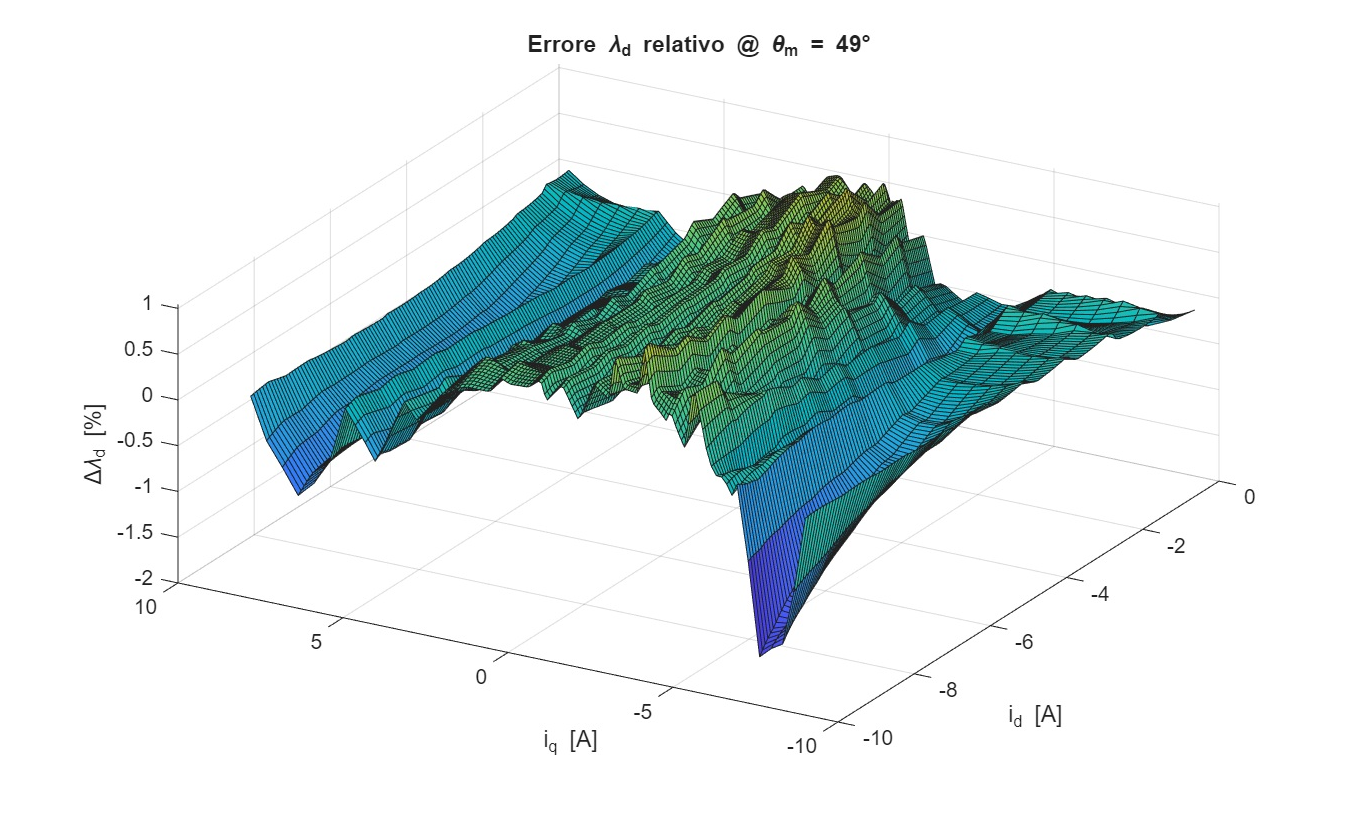
\includegraphics[height=8 cm]{immagini/errori_mappa_flusso/relativo/errore_relativo_mappe_flusso_D_xcorrenti_DEPT.pdf}
    \caption{Mappa dell'errore relativo su $\lambda_d$ (primo tentativo).}
    \label{fig:errore_relativo_mappe_flusso_D_xcorrenti_DEPT}
\end{figure}


\begin{figure}
\centering
    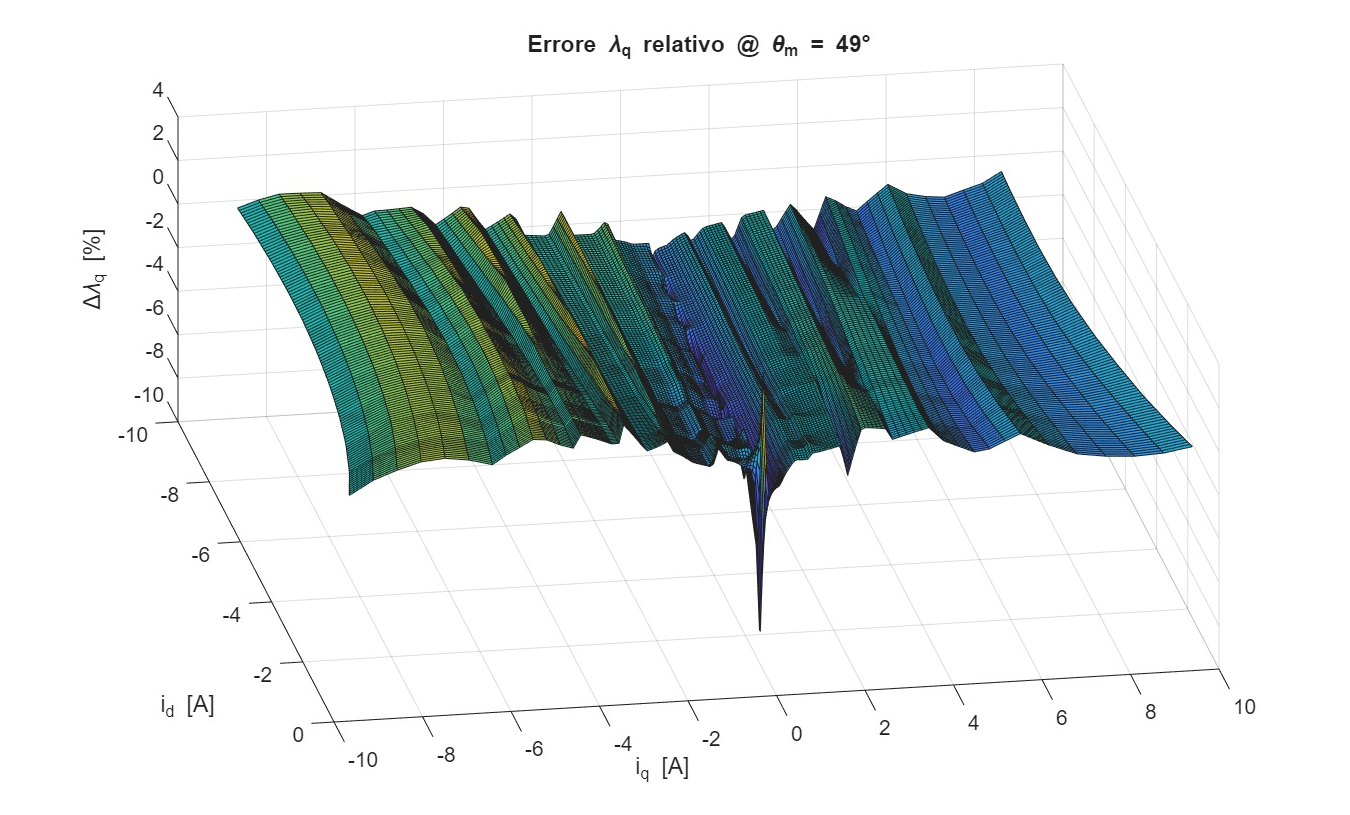
\includegraphics[height=8 cm]{immagini/errori_mappa_flusso/relativo/errore_relativo_mappe_flusso_Q_xcorrenti_DEPT.pdf}
    \caption{Mappa dell'errore relativo su $\lambda_q$ (primo tentativo).}
    \label{fig:errore_relativo_mappe_flusso_Q_xcorrenti_DEPT}
\end{figure}

\begin{figure}
\centering
    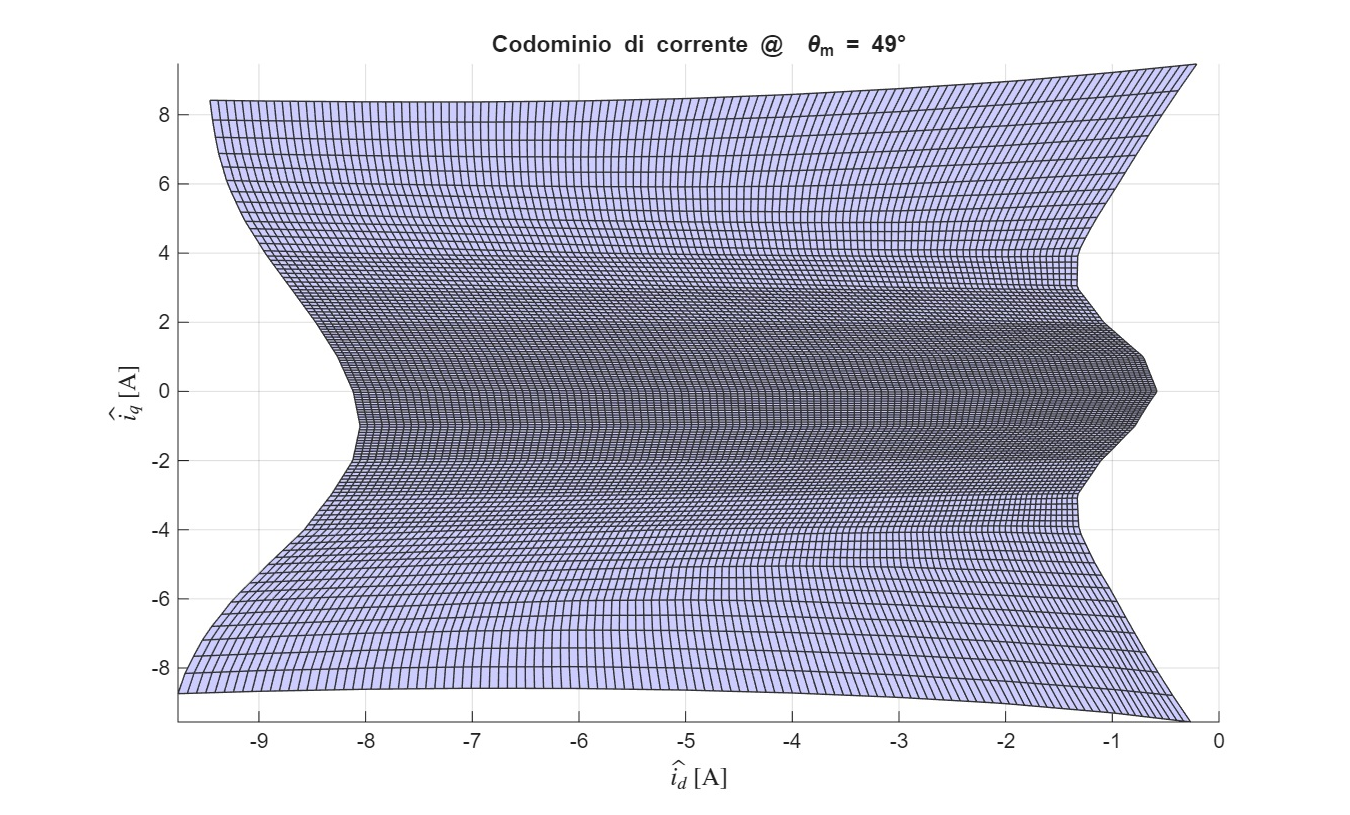
\includegraphics[height=8 cm]{immagini/errori_mappa_flusso/mappe_griglia/Mappa_correnti_UnicoColore_dense.pdf}
    \caption{Rappresentazione grafica del codominio di corrente (primo tentativo).}
    \label{fig:Mappa_lambdaD_UnicoColore_dense}
\end{figure}

\subsection{Infittimento della griglia di corrente}
Per diminuire tale errore si è infittita artificialmente la griglia di corrente delle mappe dirette di flusso, ovvero le mappe che vengono fornite alla funzione di inversione.
 In questo modo l'interpolatore \texttt{scatteredinterpolant} viene costruito a paritre da un maggior numero di punti. Si è osservato come ciò migliora considerevolmente l'accuratezza dell'inversione (Figure \ref{fig:errore_relativo_mappe_flusso_D_xcorrenti_dense} e \ref{fig:errore_relativo_mappe_flusso_Q_xcorrenti_dense}). 
Tuttavia, tale mappa inversa non comprende i valori di corrente prossimi a zero. Si veda a tal proposito la Figura \ref{fig:Mappa_lambdaD_UnicoColore_dense}. I nodi di tale grafico sono  tutti i punti di corrente associati alla griglia di flusso della mappa inversa. La griglia di flusso è costituita da tutte le combinazioni degli elementi dei vettori di flusso $\lambda_d$ e $\lambda_q$ che costituiscono le coordinate della mappa inversa.

\begin{figure}
\centering
    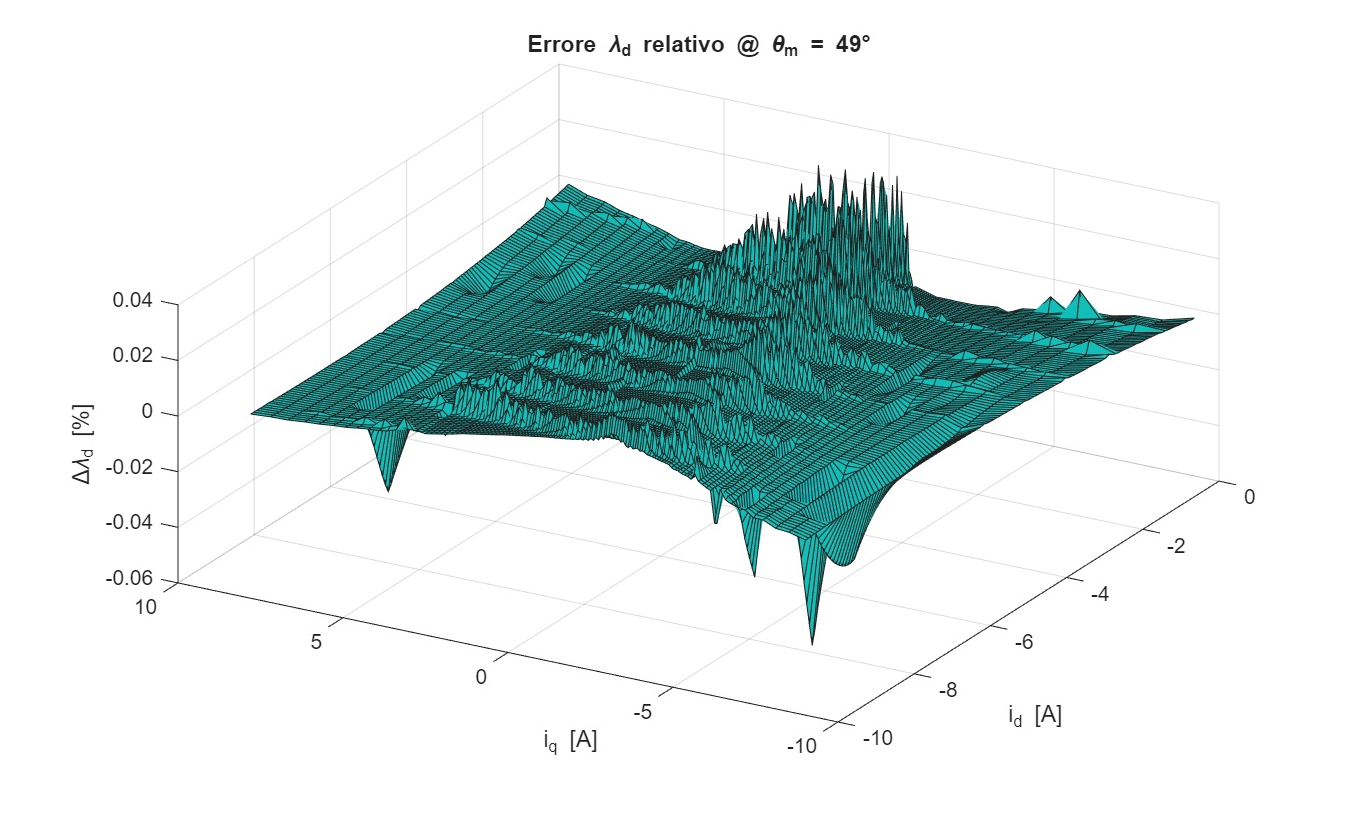
\includegraphics[height=8 cm]{immagini/errori_mappa_flusso/relativo/errore_relativo_mappe_flusso_D_xcorrenti_dense.pdf}
    \caption{Mappa dell'errore relativo su $\lambda_d$ con estensione dei vincoli di flusso.}
    \label{fig:errore_relativo_mappe_flusso_D_xcorrenti_dense}
\end{figure}


\begin{figure}
\centering
    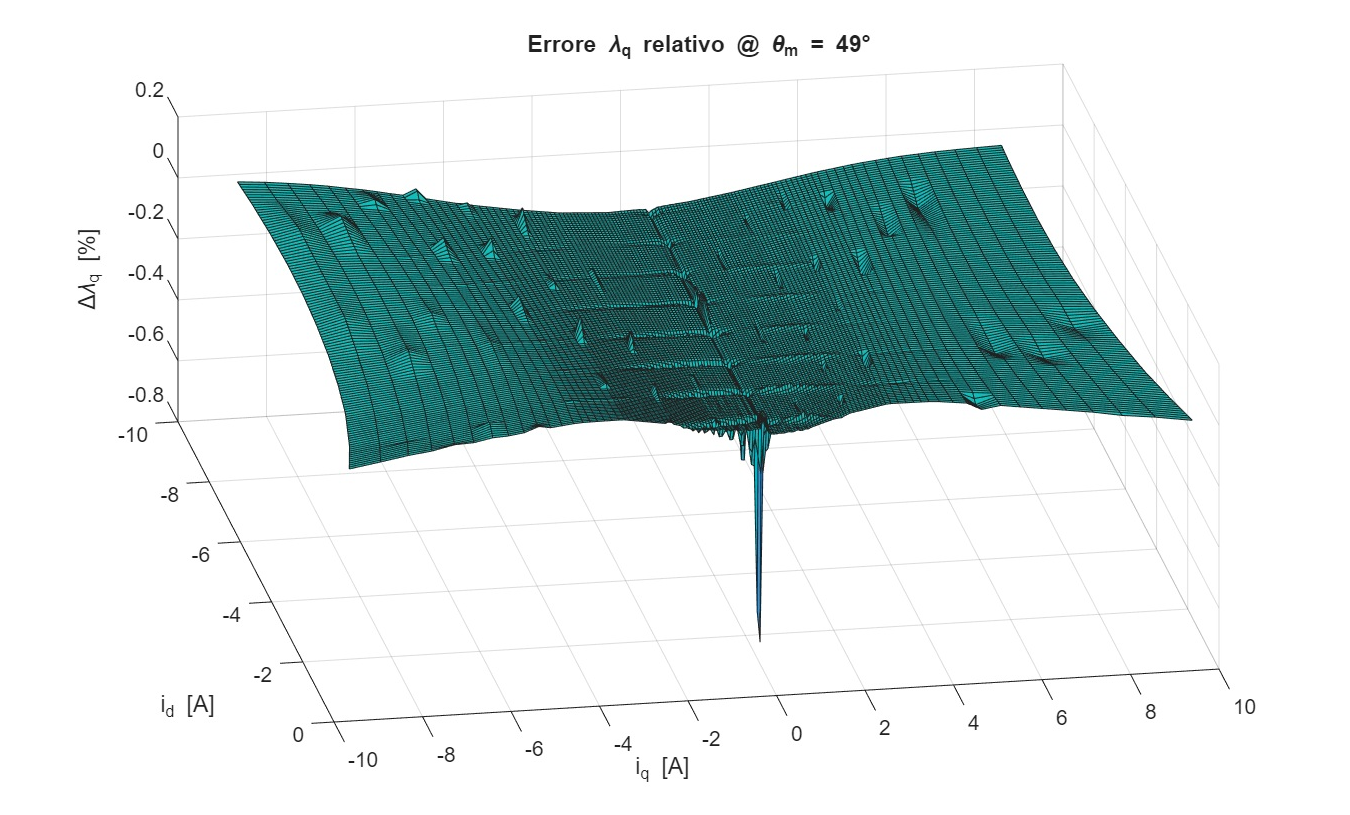
\includegraphics[height=8 cm]{immagini/errori_mappa_flusso/relativo/errore_relativo_mappe_flusso_Q_xcorrenti_dense.pdf}
    \caption{Mappa dell'errore relativo su $\lambda_q$ con infittimento della griglia.}
    \label{fig:errore_relativo_mappe_flusso_Q_xcorrenti_dense}
\end{figure}

\subsection{Infittimento della griglia e estensione dei vincoli di flusso}
Analizzando la stima del flusso per certi punti operativi, si è notata la presenza di un errore significativo di stima.\\
Questa inaccuratezza è stata ricondotta al fatto che l'estremo superiore del vettore  di flusso $\lambda_d$ risulta essere inferiore rispetto al flusso massimo associato a certi punti operativi. Ciò è vero, per esempio, per corrente nulla dove il flusso $\lambda_d$ è  massimo.\\
Pe aumentare l'accuratezza si è provato ad aumentare il range del dominio del flussi $\lambda_d$ e $\lambda_q$ della mappa invertita (Figure \ref{fig:errore_relativo_mappe_flusso_D_xcorrenti_ext} e \ref{fig:errore_relativo_mappe_flusso_Q_xcorrenti_ext}). 
Tuttavia, ciò comporta un aumento significativo dell'errore per correnti prossime a zero. La ragione di questo comportamento, come già discusso nel Paragrafo \ref{sec:limiti_dominio_flusso}, è che si introducono dei punti spuri nella stima del flusso. A una coppia di elementi dei vettori di flusso potrebbe non essere associato nessun valore di corrente nella mappa diretta. L'interpolatore quindi associa a tali valori di flusso dei valori di corrente irrealistici. \\
Ciò conferma che è necessario agire sulla mappa diretta di input alla funzione di inversione.





\begin{figure}
\centering
    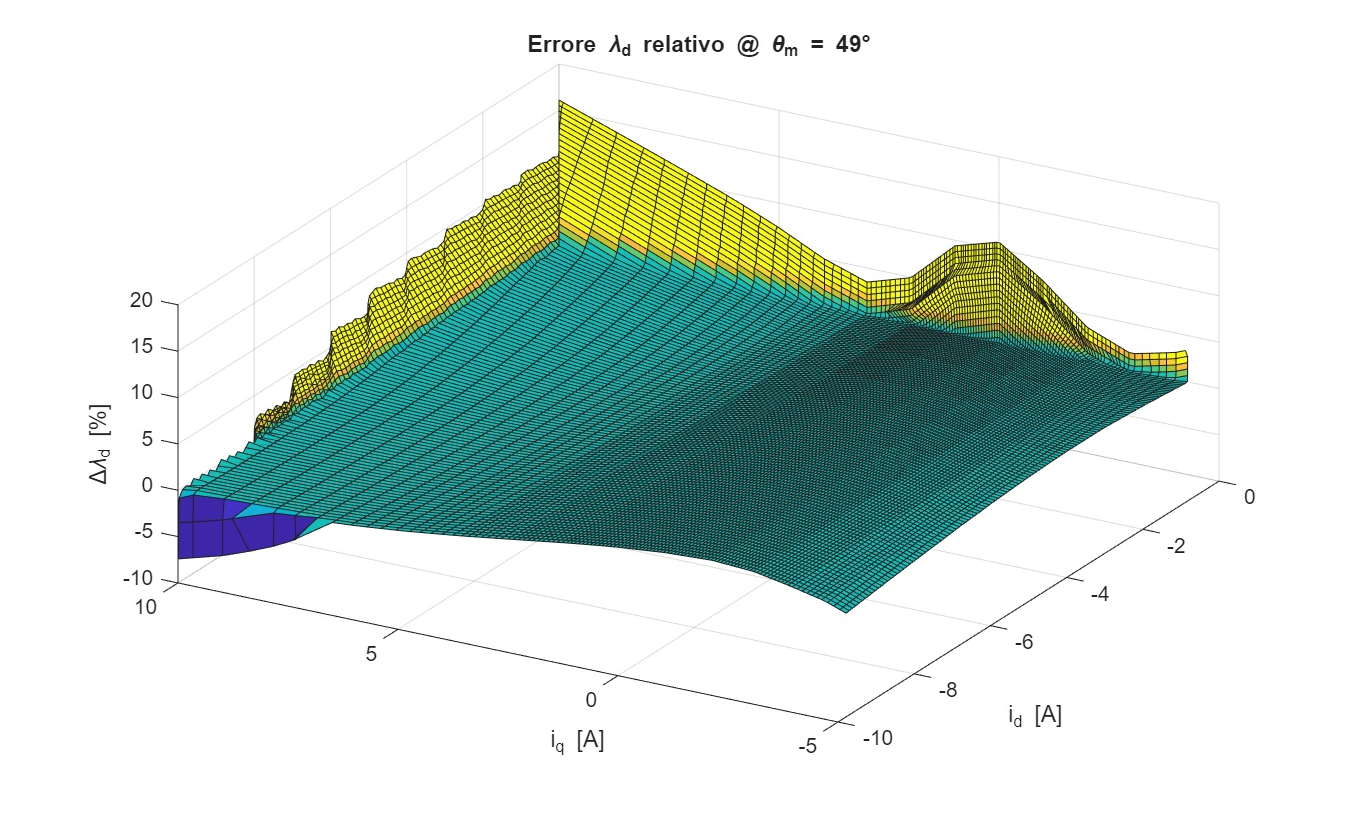
\includegraphics[height=8 cm]{immagini/errori_mappa_flusso/relativo/errore_relativo_mappe_flusso_D_xcorrenti_ext.pdf}
    \caption{Mappa dell'errore relativo su $\lambda_d$ con estensione dei vincoli di flusso.}
    \label{fig:errore_relativo_mappe_flusso_D_xcorrenti_ext}
\end{figure}


\begin{figure}
\centering
    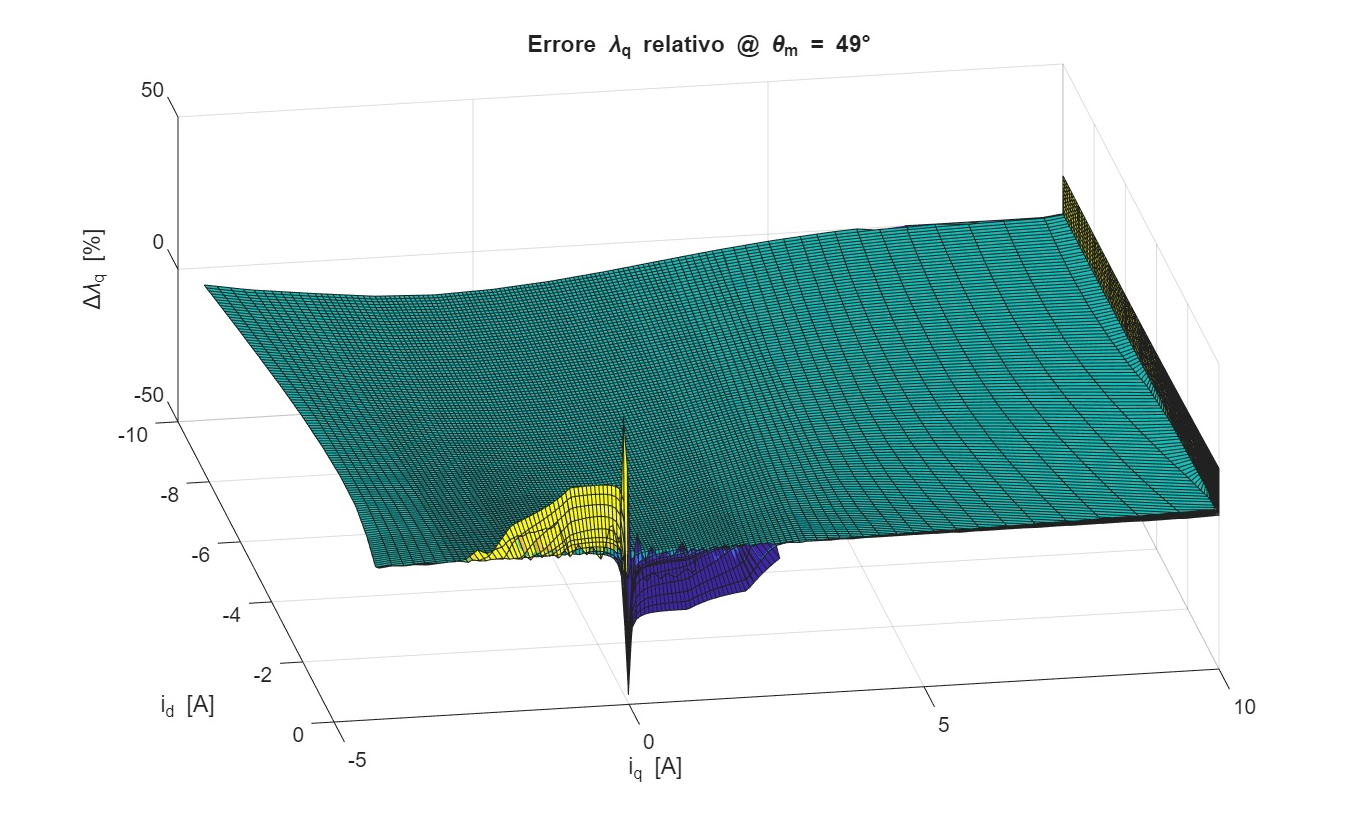
\includegraphics[height=8 cm]{immagini/errori_mappa_flusso/relativo/errore_relativo_mappe_flusso_Q_xcorrenti_ext.pdf}
    \caption{Mappa dell'errore relativo su $\lambda_q$ con estensione dei vincoli di flusso.}  \label{fig:errore_relativo_mappe_flusso_Q_xcorrenti_ext}
\end{figure}






\subsection{Estensione del dominio di corrente della mappa diretta di flusso con infittimento della griglia}
Per cercare di ridurre l'errore, si è espanso il dominio della mappa di corrente diretta iniziale anche per valori positivi di $i_d$ (Figure \ref{fig:errore_relativo_mappe_flusso_D_xcorrenti_positive} e \ref{fig:errore_relativo_mappe_flusso_Q_xcorrenti_positive}).\\ Il range della corrente della mappa diretta risulta così: 
$i_d \in [-8,\ 2] \ A$ e $i_q \in [-8,\ 8] \ A$.\\
In questo modo cambiano anche i vincoli della corrente, stabiliti utilizzando il procedimento del Paragrafo \ref{sec:limiti_dominio_flusso}. Tali vincoli risultano infatti pari a $0.0871 \ T$ e $0.2515 \ T$ per il flusso $\lambda_d$ e pari a $-0.5196 \ T$ e $0.5199 \ T$ per il flusso $\lambda_q$.
Si sono modificati anche i vincoli superiori di $i_d$ e $i_q$, dato che, essendo la corrente nominale pari a $4.2\ A$, avere un range troppo ampio risulta superfluo.\\
 Come si può notare in questo modo il codominio di corrente copre anche i valori intorno allo 0 (Figura \ref{fig:Mappa_lambdaD_UnicoColore_positive}). 



\begin{comment}

Si è provato ad estendere quindi il dominio del flusso oltre i limiti imposti in precedenza. Tuttavia, questa procedura comporta notevoli errori di stima vicino allo zero (Figura \ref{fig:errore_relativo_mappe_flusso_D_xcorrenti_ext}). 10pt
\end{comment}



\begin{comment}
\subsection{Valutazioni dei risultati ottenuti tramite la mapp inversa}
Nonostante la mappa inversa ottenuta dall'estensione della griglia di corrente iniziale risulti la più accurata, è ancora presente un errore di stima.\\
Per visualizzare tale errore, si è riportato a titolo esempleficativo un confronto tra il flusso reale e il flusso ottenuto implementando la mappa inversa per un dato punto operativo di corrente.
\end{comment}
\begin{figure}
\centering
    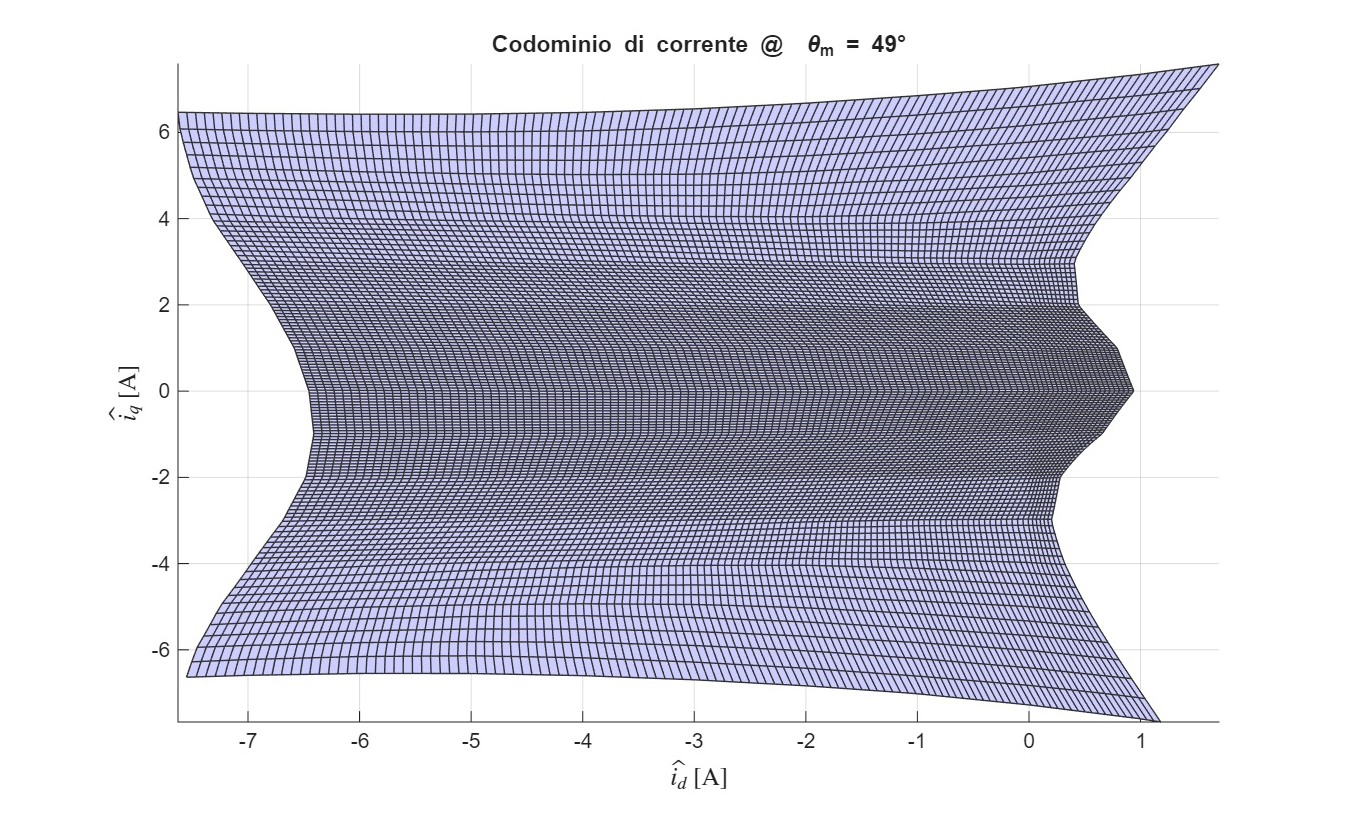
\includegraphics[height=8 cm]{immagini/errori_mappa_flusso/mappe_griglia/Mappa_correnti_UnicoColore_positive.pdf}u
    \caption{Rappresentazione grafica del codominio di corrente (quarto tentativo).}
    \label{fig:Mappa_lambdaD_UnicoColore_positive}
\end{figure}


\begin{figure}
\centering
    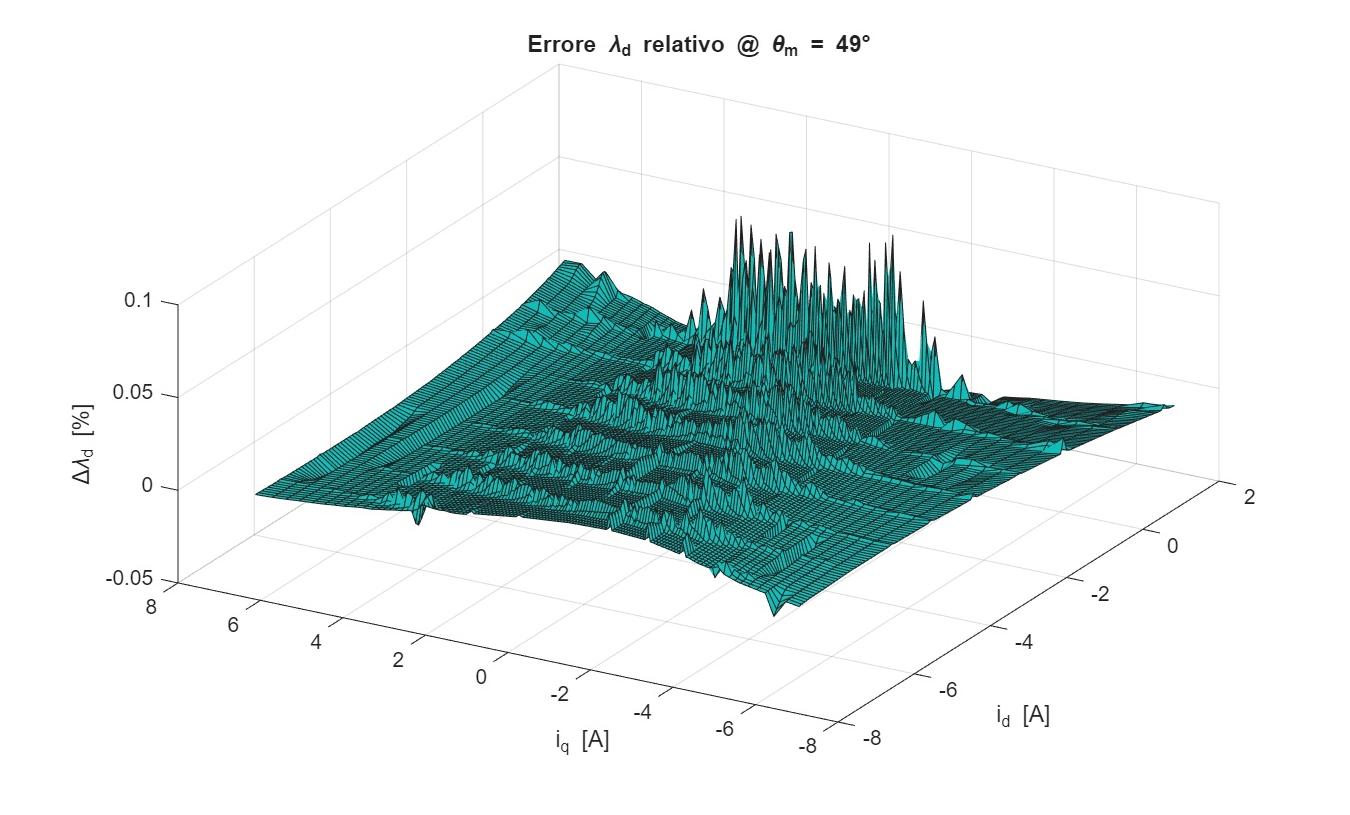
\includegraphics[height=8 cm]{immagini/errori_mappa_flusso/relativo/errore_relativo_mappe_flusso_D_xcorrenti_positive.pdf}
    \caption{Mappa dell'errore relativo su $\lambda_d$ con range positivo di corrente.}
    \label{fig:errore_relativo_mappe_flusso_D_xcorrenti_positive}
\end{figure}


\begin{figure}
\centering
    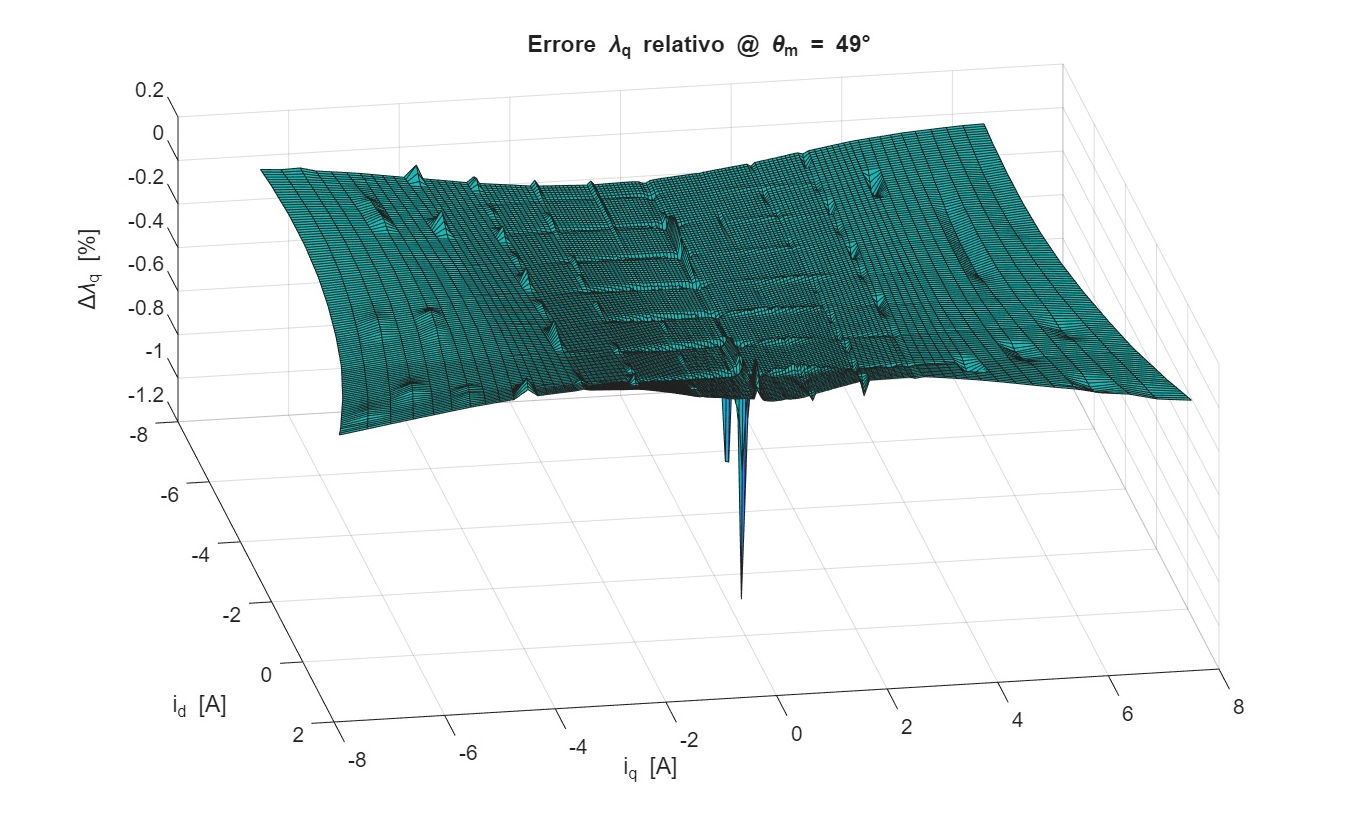
\includegraphics[height=8 cm]{immagini/errori_mappa_flusso/relativo/errore_relativo_mappe_flusso_Q_xcorrenti_positive.pdf}
    \caption{Mappa dell'errore relativo su $\lambda_q$ con range positivo di corrente.}  
    \label{fig:errore_relativo_mappe_flusso_Q_xcorrenti_positive}
\end{figure}

